\documentclass[simplex.tex]{subfiles}
% NO NEED TO INPUT PREAMBLES HERE
% packages are inherited; you can compile this on its own

\onlyinsubfile{
\title{NeuroData SIMPLEX Report: Subfile}
}

\begin{document}
\onlyinsubfile{
\maketitle
\thispagestyle{empty}

The following report documents the progress made by the labs of Randal~Burns and Joshua~T.~Vogelstein at Johns Hopkins University towards goals set by the DARPA SIMPLEX grant.

%%%% Table of Contents
\tableofcontents

%%%% Publications
\bibliographystyle{IEEEtran}
\begin{spacing}{0.5}
\section*{Publications, Presentations, and Talks}
%\vspace{-20pt}
\nocite{*}
{\footnotesize	\bibliography{simplex}}
\end{spacing}
%%%% End Publications
}

\subsection{Randomer Forest (RerF)}
Most recently, we compared classification performances of RF, RerF, RR-RF, and XGBoost on 119 benchmark datasets. RR-RF is identical to RF except that
the data is randomly rotated prior to building each tree. XGBoost is a
computationally efficient implementation of gradient boosted trees and
has been the winner of many recent Kaggle competitions. For each
dataset, for each algorithm, error was subtracted by that of RF and
normalized by the chance probability of error. These
normalized relative errors were then binned and the counts in each bin
were computed. The y-axis represents the bins. Color indicates how many
times the normalized relative error of an algorithm fell into a
particular bin. For instance, the figure shows that RerF had a
normalized relative error 0.05 to 0.10 less than that of RF on
approximately 15 datasets. The ``0 to 0'' bin indicates the number of
times the normalized relative error was exactly 0. Overall the figure
indicates that RerF rarely loses to RF by much and frequently does
substantially better. RR-RF and XGBoost, on the other hand, frequently
perform worse than RF by a large margin.

Additionally, we have made progress towards a more scalable implementation of RerF in R. The previous port of RerF to R rotated input data at the tree level instead 
of at the more desired node level.  The new port of RerF now rotates at the
node level.  The change to R will allow a fast RerF implementation by 
integrating the algorithm into FlashR.

\begin{figure}[h!]
\begin{cframed}
\centering
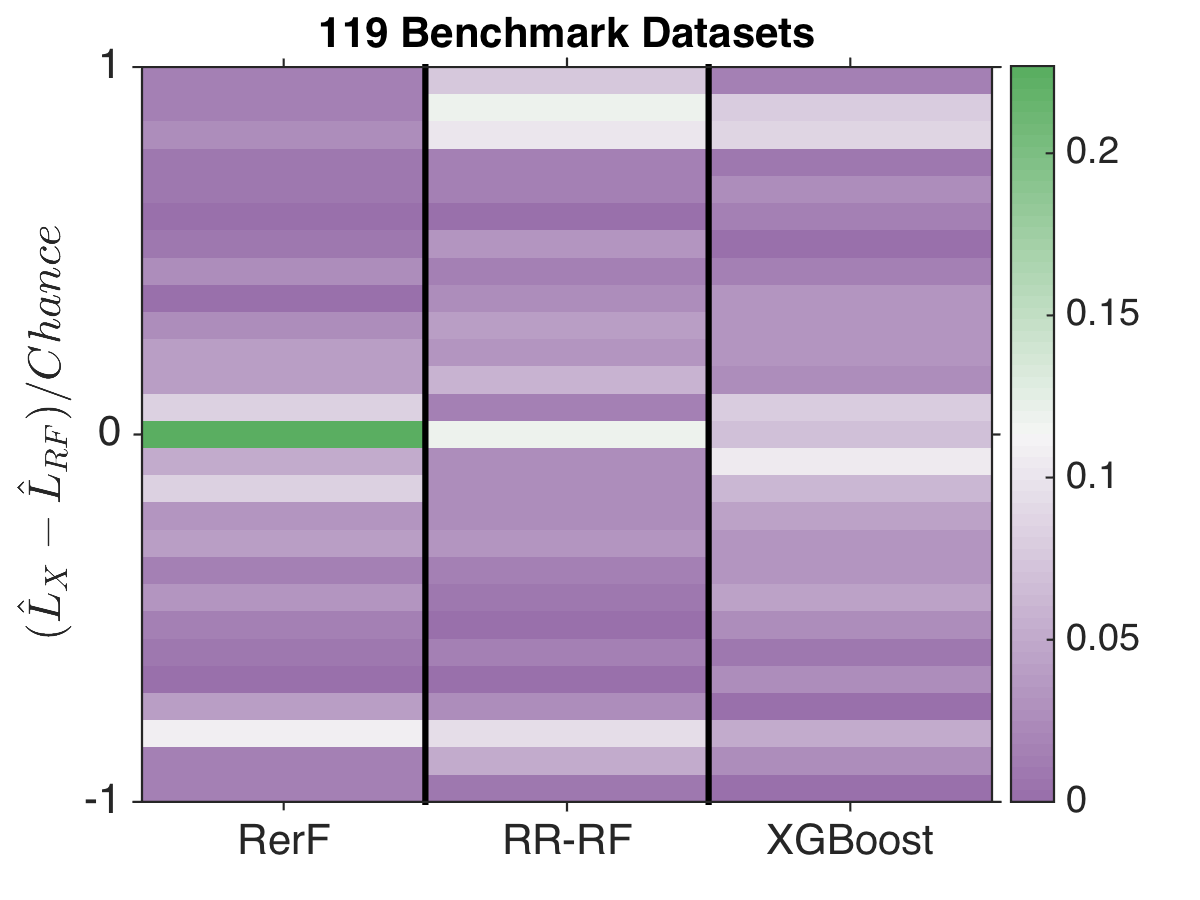
\includegraphics[height=0.5\textheight]{../../figs/rerF_benchmark.png}
\caption{
Classification performances of RF, RerF, RR-RF, and XGBoost
on 119 benchmark datasets.
}
\label{fig:RefF3}
\end{cframed}
\end{figure}

\end{document}
